\chapter{Intrinsic network architecture and skilled reading}

\section{Motivation}

% Intrinsic network architecture
In the functional connectivity literature, researchers generally refer to two types of connectivity: intrinsic (or resting-state) connectivity and task-evoked connectivity. Network organization at rest is thought to be highly similar across people \citep{Damoiseaux2006}, and the pattern of connectivity within an individual is consistent over periods of time in excess of three years \citep{Choe2015}. It is thought that this stability may reflect a history of co-activation among brain regions that occurs over time \citep{Power2010}, and it is closely tied to patterns of white matter anatomical connectivity \citep{Honey2009}. As discussed in the introduction, a major feature of intrinsic network architecture is that of resting-state networks (RSNs). RSNs can be identified on an individual basis \citep{Laumann2015} and are composed of brain regions that tend to function as a unit \citep{DeLuca2006, Smith2009}. This functional subdivision of the whole-brain network is hypothesized to provide a neural substrate for the diversity of cognitive functions in which people engage \citep{Yeo2014}.

% Pivot to individual differences in RSNs
Despite the overall stability across individuals, variations in network architecture have been noted. For example, differences have been observed in individuals who exhibit variation in executive functions \citep{Reineberg2015, Tian2015} and in individuals with genetic susceptibility to Alzheimer’s disease \citep{Trachtenberg2012}. Consequently, variation in RSNs are likely to be stable measures of individual differences. To date, however, their relationship to other cognitive domains, and in particular reading, is not well understood.  Given that large-scale networks underlie a variety of cognitive functions, it follows that individual variation within certain reading-related networks and the interaction among RSNs could be linked to varying reading abilities. The existence of these associations can be used to not only predict cognitive and academic functioning at the level of the individual, but also to allocate treatments, model developmental trajectories, or predict  responses to intervention \citep{Mattfeld2014, Crowther2015, Whitfield-Gabrieli2016}. 

% Graph measures of connectivity
A major question is how best to model RSN properties so that they are both sensitive to network composition (e.g. default mode, fronto-parietal) and globally representative. In some of the initial and influential connectomics studies, whole-brain measures such as the ``efficiency'' or ``characteristic path length'' were used to show a relationship between intelligence and network architecture \citep{Stam2014}. On the other hand, other studies have investigated the roles of individual nodes in the whole-brain network -- to identify individual hub regions, for example \citep{Betzel2013}. Although useful, neither of these sets of measures model the composition of \textit{functional systems}, i.e. RSNs. Connectivity measures related to a specific region such as the visual word form area, might be sensitive to differences in auditory-visual processing, but do not reflect the organization of the visual system at large \citep{Rubinov2010}. Employing measures that are sensitive to regional variation, such as modularity and the participation coefficient, could better clarify drivers of individual differences in specific cognitive domains such as reading \citep{Cao2016}. One limitation is that these measures require a definite parcellation of the brain into RSNs, which has only become possible as the initial exploratory and descriptive studies have been done.

% Global measures, the reading system
We hope to better understand how variations in connectivity within and between RSNs is related to individual differences in reading skill. In general, skilled reading is associated with left hemisphere language and word recognition regions (left inferior frontal, supramarginal and occipito-temporal regions), and fronto-parietal regions supporting attention \citep{Paulesu2014}. The brain regions supporting reading do not, however, form a unique, fundamental network. Instead, reading appears to rely on the reconfiguration and integration of multiple, more fundamental brain networks \citep{Koyama2010, Vogel2013}. Indeed, emerging research suggests that functional connectivity indices are associated with differences in reading skill. Struggling readers, such as those with dyslexia, exhibit decreased connectivity between visual association areas and prefrontal attention areas, increased right hemisphere connectivity, and reduced connectivity to occipito-temporal cortex compared to non-impaired readers \citep{Finn2014}. In typically developing readers, Koyama and colleagues found increased positive connectivity among language regions was associated with increased word reading ability \citep{Koyama2011}, and recent studies suggest that interventions designed to enhance reading skill can increase the correlations between visual and frontal executive areas \citep{Horowitz-Kraus2015}. 

% RSN measures that might be useful
Although most cognitive functions are relevant to reading in some way, the RSNs most associated with primary reading subprocesses are the fronto-parietal, ventral attention, and visual RSNs. In addition to the intensity and composition of these networks, coordination between these brain areas and others are also likely to play a role in differentiating higher from lower performing readers. A separate study by Koyama and colleagues found that increased reading ability was associated with increased negative connectivity between reading regions and regions of the default mode network \citep{Koyama2013}, a network typically implicated in internally-directed thinking \citep{Andrews-Hanna2014}. This negative relationship between the default and reading networks echoes work showing that increased anti-correlated activity between the default network and regions specialized for cognitive function, such as those involved in attention, inhibitory control, and working memory is associated with individuals who display higher performance. We expect, then, that there will be both regional and global effects of network architecture on reading skill.

% Study setup
Because of its stability and close ties to structure, understanding the degree of variability in intrinsic network architecture will serve as an excellent starting point for our aims. An in depth examination of how behavioral indices of reading relate to various properties of RSNs has not been previously reported, except within our own group \citep{Bailey2018}. First, we validate the existence of a small-world architecture in these subjects, and that the network parcellation is appropriate for them. Second, we determine whether global measures of network architecture, including modularity, participation coefficient and path length, are related to reading skill. Finally, we determine which RSNs drive the relationship between connectivity and reading skill. To address each of these questions, we analyze resting-state fMRI in developing readers, which has the further potential benefit of being able to be performed before children even start reading.


\section{Methods}

The following methods detail the current study's protocol and analytic approach. Because the following chapters borrow heavily from the methods described below, they are explained here in detail. 

\subsection{Participants}

Participants were drawn from the fourth wave of a larger, longitudinal study investigating the neurobiological bases of reading comprehension. In total, 52 children completed scans and a subset of these met the motion and attention thresholds described below.

All participants were native English speakers with normal hearing and normal or corrected vision, and no history of major psychiatric illness or traumatic brain injury/epilepsy. Subjects had no history of a developmental disability or contra-indication to MRI.  Each participant gave written consent at the beginning of the study, with procedures carried out in accordance with Vanderbilt University’s Institutional Review Board.

\begin{table}
    \renewcommand{\tabcolsep}{0.09cm}
    \centering
    \begin{tabular}{lc}
\toprule 
Measure & Subjects \\ 
\midrule 
No. Participants				& 42 \\ 
No. Scan Runs					& 164 \\ 
Gender  						& 25 F \\ 
Age at Scan 					& 10.5 (0.3)  \\ 
WASI Full-Scale IQ  			& 111.0 (16.2) \\ 
TOWRE - Total Word Efficiency 	& 104.6 (18.5) \\ 
\bottomrule 
\end{tabular}
    \caption[Participant demographics for Study 1]{Demographics and mean test scores for Study 1 participants are described here. For continuous data, the standard deviation is enclosed in parentheses.}
    \label{table:ch2-participants}
\end{table}

In addition to having an MRI scan, participants completed cognitive tests, including the Wechsler Abbreviated Scale of Intelligence (WASI) \citep{Kaplan1999}, the Test of Word Reading Efficiency (TOWRE) \citep{Torgesen2012}, the Woodcock Reading Master Tests (WRMT) \citep{Woodcock1998}, and the Gates-MacGinitie Reading Comprehension test \citep{MacGinitie2000}, among others. Demographics and selected test data are summarized in Table \ref{table:ch2-participants}.

\subsection{MRI acquisition and preprocessing}

Imaging was performed on a Philips Achieva 3T MR scanner with a 32-channel head coil. Functional images were acquired using a gradient echo planar imaging sequence with 40 (3 mm thick) slices with no gap. Resting-state fMRI scans consisted of 190 dynamic volumes. Slices were parallel to the anterior-posterior commissure plane. Imaging parameters for functional images included: TE = 30 ms; FOV = 240 x 240 x 120 mm\textsuperscript{3}; flip angle = 75\degree; TR = 2200 ms; and 3 mm\textsuperscript{3} isotropic voxels.

\begin{figure}[t]
    \centering
    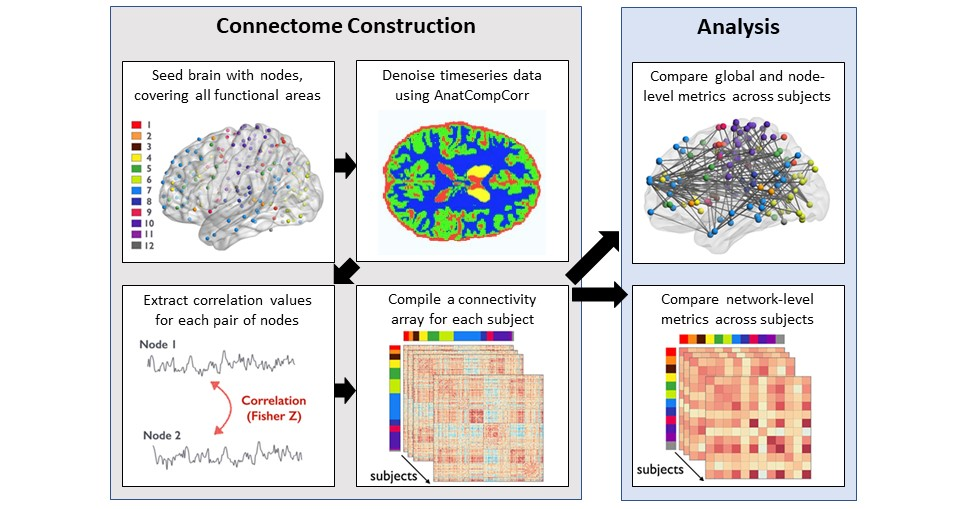
\includegraphics[width=6in]{ch2-connectome-methods}
    \caption[Schematic for connectome construction]{Connectomes are constructed from resting-state fMRI in the following steps: slice-timing correction, rigid-body motion correction, boundary-based registration to a T1-weighted anatomical image, and normalization to MNI 152 template. The timseries for 264 nodes are then extracted and denoised using signal from non-neural tissue, continuous motion parameters and outliers. A pair-wise connectivity matrix is then calculated and thresholded at multiple different thresholds, then analyzed at the global-, RSN-, or node-level. Figure adapted from \citep{Yang2018}.}
    \label{fig:ch2-connectome-methods}
\end{figure}

Whole-brain fMRI analyses were performed using tools from the FMRIB Software Library (version 5.0.9). For each session, the following pre-processing steps were performed:  slice-time correction, motion correction to the initial fMRI volume, boundary-based registration to the subject's structural image, and normalization to 2 mm MNI 152 standard space. To mitigate the effects of motion on our analyses, we regressed out 6 continuous motion parameters and scrubbed out outlier volumes. We defined an outlier volume as any in which the root-mean-square framewise displacement exceeded 0.7 mm. Because head motion can be a major confound for connectivity analyses, we removed scan runs where more than 20 percent of the fMRI volumes were outliers.

\subsection{Network construction}

To investigate whole-brain patterns of connectivity with minimal investigator bias, we selected 264 nodes \textit{a priori} whose connectivity properties have been extensively analyzed in previous works \citep{Power2011, Power2013, Cole2014}. The node set samples the entire brain, and nodes were selected based on their involvement in a diversity of cognitive tasks. Each node was assigned to one of 13 RSNs based on a previous study \citep{Power2013}. Approximately 10 percent of the nodes did not have a stable assignment in the original paper; for the present analyses, these nodes were excluded from graph theory calculations but included in network formation. A description of the 13 networks and their sizes is provided in Table \ref{table:ch2-power-nodes}. 

\begin{table}[t]
	\renewcommand{\tabcolsep}{0.09cm}
	\centering
	\begin{tabular}{lcc}
\toprule 
Suggested RSN & Abbreviation & Nodes \\ 
\midrule 
\textit{Sensory} & & \\
	\hspace{3pt}Auditory  			&  AUD & 13 \\ 
	\hspace{3pt}Somatomotor (Hand)	&  SOH & 30 \\
	\hspace{3pt}Somatomotor (Mouth)	&  SOM & 5 \\
	\hspace{3pt}Visual	 			&  VIS & 31 \\ 
\textit{Attention} & & \\
	\hspace{3pt}Dorsal attention  	&  DAN & 11	\\ 
	\hspace{3pt}Salience		  	&  SAL & 18 \\ 
	\hspace{3pt}Ventral attention  	&  VAN & 9 \\ 
\textit{Executive / Associative} & & \\
	\hspace{3pt}Cingulo-opercular 	& CON & 14 \\ 
	\hspace{3pt}Default mode		& DMN & 58 \\
	\hspace{3pt}Fronto-parietal  	& FPN & 25 \\ 
	\hspace{3pt}Memory retrieval	& MEM & 5 \\
\textit{Other} & & \\
	\hspace{3pt}Cerebellar			& CER & 4  \\
	\hspace{3pt}Subcortical			& SUB & 13 \\
	\hspace{3pt}Not assigned 		& UNC & 28 \\ 
\bottomrule 
\end{tabular}
	\caption[List of resting-state networks]{List of networks used in connectivity analyses and the number of nodes affiliated with each. Although alternative parcellations of the node set are possible, we elected to use those network assignments suggested in \citep{Power2013}.}
	\label{table:ch2-power-nodes}
\end{table}

Connectivity analysis was performed in the CONN toolbox \citep{WhitfieldGabrieli2012}. Resting-state fMRI data were high-pass filtered at 0.008 Hz, motion-corrected, co-registered to a structural image, normalized to MNI space and smoothed by a 5 mm FWHM spherical kernel. BOLD signal timeseries were corrected using ``anatCompCorr'', which uses signal from white matter tissue and cerebrospinal fluid areas to reduce noise not related to brain activity \citep{Chai2012}. We also regressed out 12 continuous measures of motion and all outlier timepoints. The timeseries was then high-pass filtered at 0.01 Hz. fMRI timeseries correlations were calculated between each of the the 264 nodes, resulting in a single connectivity array for each subject at each time point. Matrices were then thresholded into binary maps by keeping the top 5 percent of connections. (To confirm that this particular threshold did not unduly influence results, we also swept results between thresholds at the top 2 percent to the top 10 percent of connections.)

\subsection{Network analyses}

The metrics of interest were network \textit{modularity}, \textit{participation coefficient} and \textit{path length} \citep{Rubinov2010}. Modularity is high in networks where nodes within the same RSN are highly connected to each other but not elsewhere. The participation coefficient, on the other hand, is high when many nodes are connected to several different RSNs. Both of these metrics relate to the integration of information between RSNs. Path length describes the distance between any two nodes on the graph. This was calculated between every node, then summed up by RSN to create a measure of network distance. These properties, and their changes within our task, were investigated at the level of connectomes, RSNs and nodes. 

% Put in a figure explaining the measures provided
\begin{figure}[t]
    \centering
    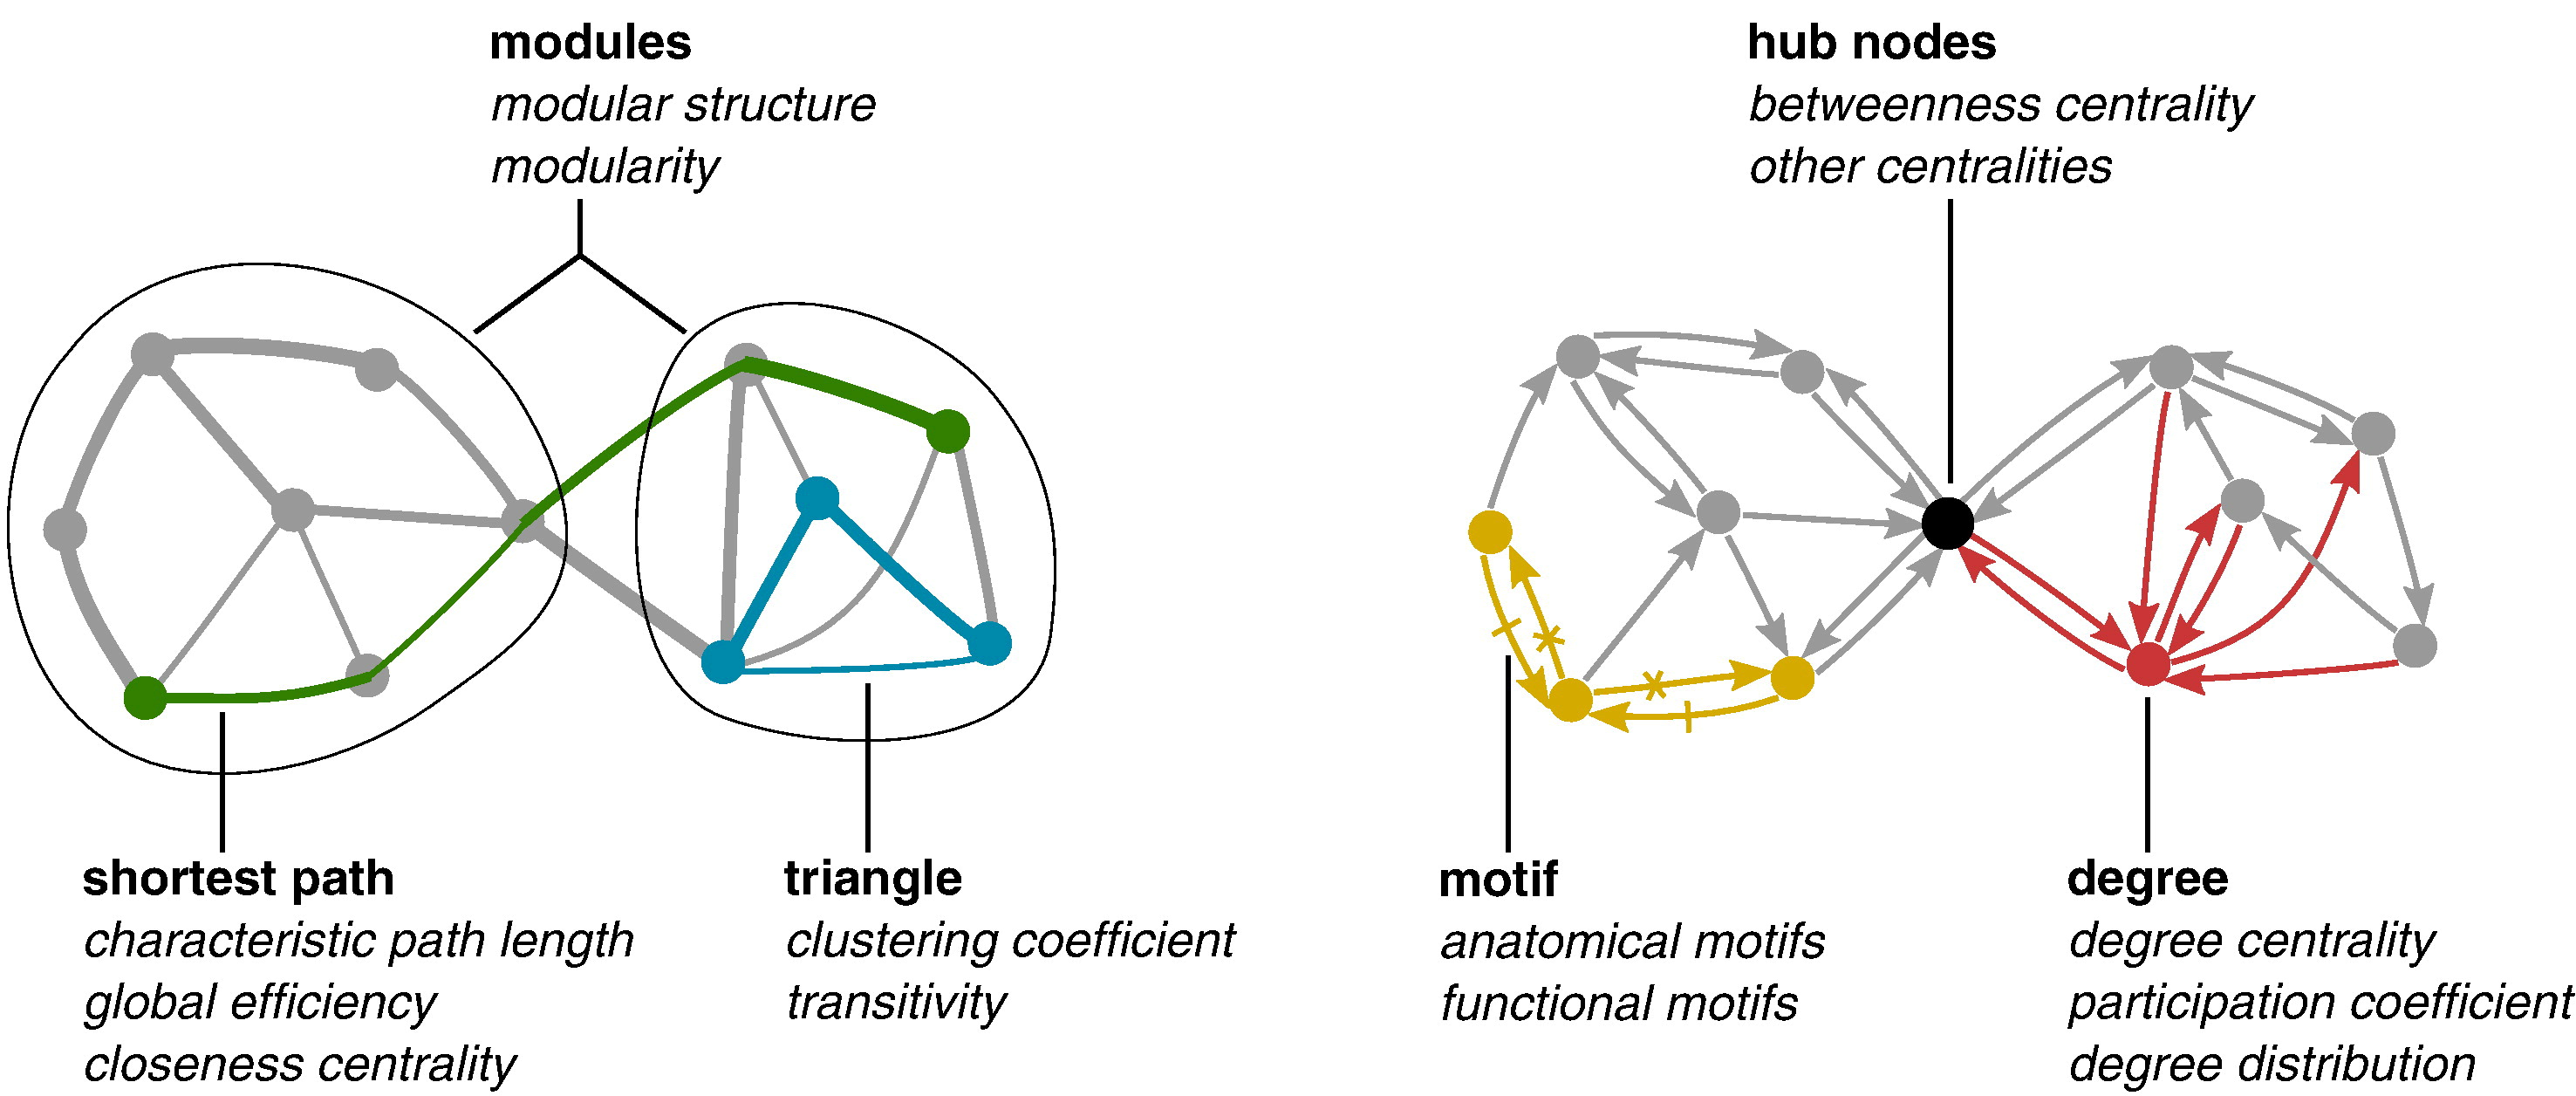
\includegraphics[width=6in]{ch2-brain-measures-diagram}
    \caption[Sampling of graph theory measures]{Sampling of graph theory measures, including those of present interest. Modularity (left, circular regions) is high in networks where nodes within the same RSN are highly connected to each other but not elsewhere. Path length describes the distance between any two nodes on the graph (left, green line). The participation coefficient, on the other hand, is high when many nodes are connected to several different RSNs (right, center node). Figure is reprinted from \citep{Rubinov2010}.}
    \label{fig:ch2-brain-measures-diagram}
\end{figure}

First, we establish the validity of the parcellation for evaluting network properties in this sample. At rest, we expect to see high modularity (greater than 0.1), low participation (less than 0.9), and a lower path length within RSNs than between them. We also expect to see moderate-sized correlations between measures, since each is measuring an aspect of network architecture related to distance between nodes.  

Next, we break each global measure down by RSN to determine how sub-systems differ in their network roles. For modularity, we report the total modularity contribution for each network. For participation coefficient and path length, we report the mean value within each network. We also investigate the measures obtained across the whole range of network-forming thresholds (retaining the top 2 to 10 percent of connections). We expect to see changes in the measures across thresholds, but ranked in a relatively stable order among the different RSNs. 

To determine the relationship between network measures and individual performance on cognitive assessments, we input each global metric into a general linear model with the Test of Word Reading Efficiency (TOWRE, total word efficiency (TWE) standard score). Models containing measures of mean framewise-displacement (motion) and the WASI Vocabulary measure were also assesed to ensure that effects were not driven by motion confounds or global measures of cognitive skill. We also examined whether there were differences in the modularity relationship between TOWRE subtests (sight word efficiency  and phonemic decoding efficiency). 

To assess whether there was an RSN-level trend in the modularity-to-reading relationship, post-hoc analyses comparing network-level modularity values to TOWRE scores were also investigated. For each node, a correlation value was calculated between its modularity contribution and TOWRE TWE scores. To evaluate significance, RSN correlations were compared to a bootstrapped distribution of 5000 correlation values generated by sampling and totaling the modularities for a random set of nodes equal in size to the selected RSN. (For example, summing modularity contributions for 31 random nodes for comparison to the visual network.)


\section{Results} 

Of the 52 subjects who completed resting-state fMRI scans, 44 met the scan quality criteria for inclusion. Connectome parcellations at the 5 percent threshold exhibited small-world properties: the mean modularity value was 0.264 (SD = 0.037), and the mean participation coefficient was 0.599 (0.052). Furthermore, the path length within RSNs was significantly lower than those between: within-community nodes took an average of 2.49 (0.141) steps to reach each other, whereas between-community nodes took an average of 3.06 (0.207) steps ($p < 0.001$, two-sample $t$-test). Furthermore, a comparison of each metric against the others shows that, while there is overlap between the measures at the global level, there is substantial variability as well (Table \ref{fig:ch2-global-graph-theory-descriptions}).

\begin{figure}[t]
    \centering
    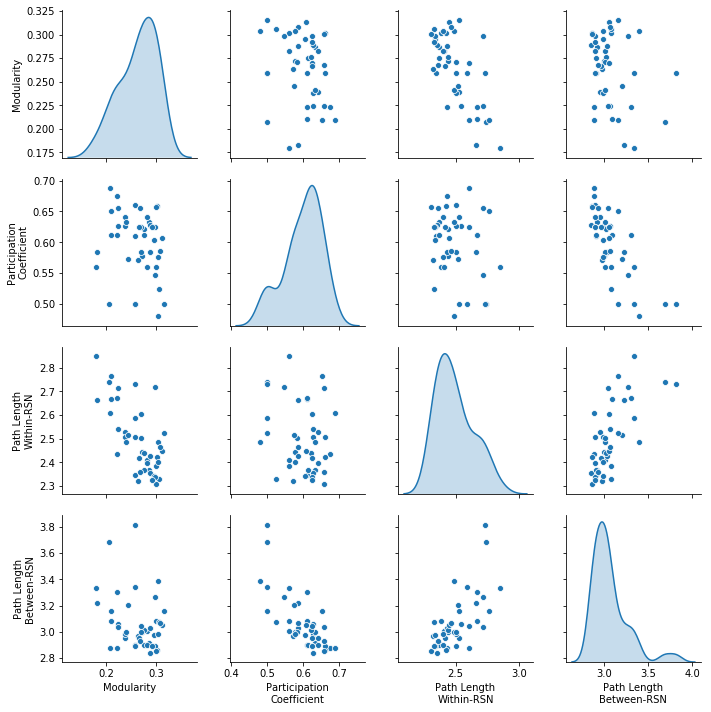
\includegraphics[width=5in]{ch2-global-graph-theory-descriptions}
    \caption[Distribution and correlations between global graph theory measures]{Distribution and correlations between the global modularity, participation coefficient and path length. Each attribute may be interpreted as a measure of connectedness between RSNs, but there is substantial variability between them.}
    \label{fig:ch2-global-graph-theory-descriptions}
\end{figure}

Figure \ref{fig:ch2-network-graph-theory-descriptions} highlights the contributions of each RSN to the graph theory measures. The visual, somatomotor, and default mode were the most modular RSNs, in part reflecting their larger size relative to others. The dorsal attention, auditory and cingulo-opercular networks were the most participatory RSNs at rest. The fronto-parietal RSN occupied an interesting place, possessing relatively high modularity but also one of the higher participation coefficients and lower global path lengths. The effect of changing thresholds had consistent effects on each measure: as more connections were included, the modularity decreased, participation coefficient increased, and path length decreased (Fig. \ref{fig:ch2-network-graph-theory-descriptions}, bottom). 

\begin{figure}[t]
    \centering
    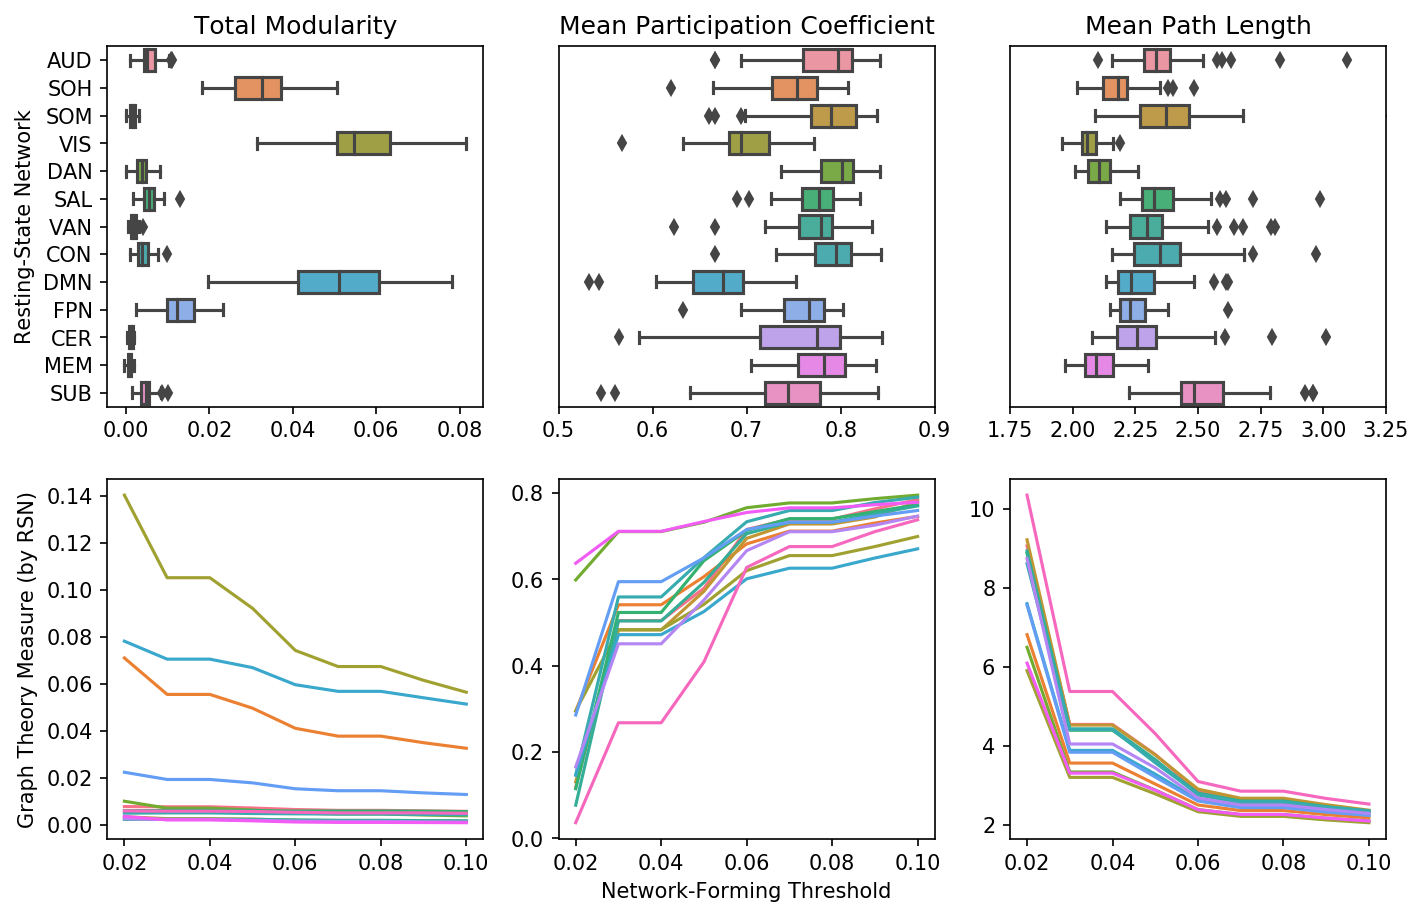
\includegraphics[width=6in]{ch2-network-graph-theory-descriptions}
    \caption[Relationships between network-level graph theory measures]{Relationships between network-level graph theory measures. Shown above are the network-level distributions of the graph theory measures when graphs are thresholded for the top 10 percent of connections (top row), and the network means as the network-forming thresholds are swept from 2 percent to 10 percent (bottom row).}
    \label{fig:ch2-network-graph-theory-descriptions}
\end{figure}

The relationships between each graph theory metric to TOWRE Total Word Efficiency scores are summarized in Table \ref{table:ch2-global-glm-results}. Global modularity, but not participation coefficient or path length, was predictive of reading skill even after controlling for mean frame-wise displacement (motion) and verbal intelligence ($Z_{TWE} = 2.536$). The direction of the relationship was positive, and it was higher for the Sight Word Efficiency subtest ($Z_{SWE} = 2.779$) than for Phonemic Decoding Efficiency ($Z_{PDE} = 2.138$), which did not reach significance when confounds were controlled. 

\begin{table}[t]
    \renewcommand{\tabcolsep}{0.09cm}
    \centering
    \begin{tabular}{lcc}
\toprule 
Independent Variable & Coeff. & $p$-value \\ 
\midrule 
\textit{Sensory} & & \\
	\hspace{3pt}Auditory  			&  AUD & 13 \\ 
	\hspace{3pt}Somatomotor (Hand)	&  SOH & 30 \\
	\hspace{3pt}Somatomotor (Mouth)	&  SOM & 5 \\
	\hspace{3pt}Visual	 			&  VIS & 31 \\ 
\textit{Attention} & & \\
	\hspace{3pt}Dorsal attention  	&  DAN & 11	\\ 
	\hspace{3pt}Salience		  	&  SAL & 18 \\ 
	\hspace{3pt}Ventral attention  	&  VAN & 9 \\ 
\textit{Executive} & & \\
	\hspace{3pt}Cingulo-opercular 	& CON & 14 \\ 
	\hspace{3pt}Default mode		& DMN & 58 \\
	\hspace{3pt}Fronto-parietal  	& FPN & 25 \\ 
	\hspace{3pt}Memory retrieval	& MEM & 5 \\
\textit{Other} & & \\
	\hspace{3pt}Cerebellar			& CER & 4  \\
	\hspace{3pt}Subcortical			& SUB & 13 \\
	\hspace{3pt}Not assigned 		& UNC & 28 \\ 
\bottomrule 
\end{tabular}
    \caption[Comparison of global graph theory metrics to reading skill]{Results for analyses comparing global graph theory metrics to reading skill.}
    \label{table:ch2-global-glm-results}
\end{table}

The relationship between modularity and TOWRE is stable across multiple thresholds (Fig. \ref{fig:ch2-global-glm-covariates-thresh}). In fact, when graph theory measures were compared to other language-related assessments, there was a trend towards a significant positive relationship between modularity and cognitive performance that was more stable than those of either the participation coefficient or global path length. 

\begin{figure}[t]
    \centering
    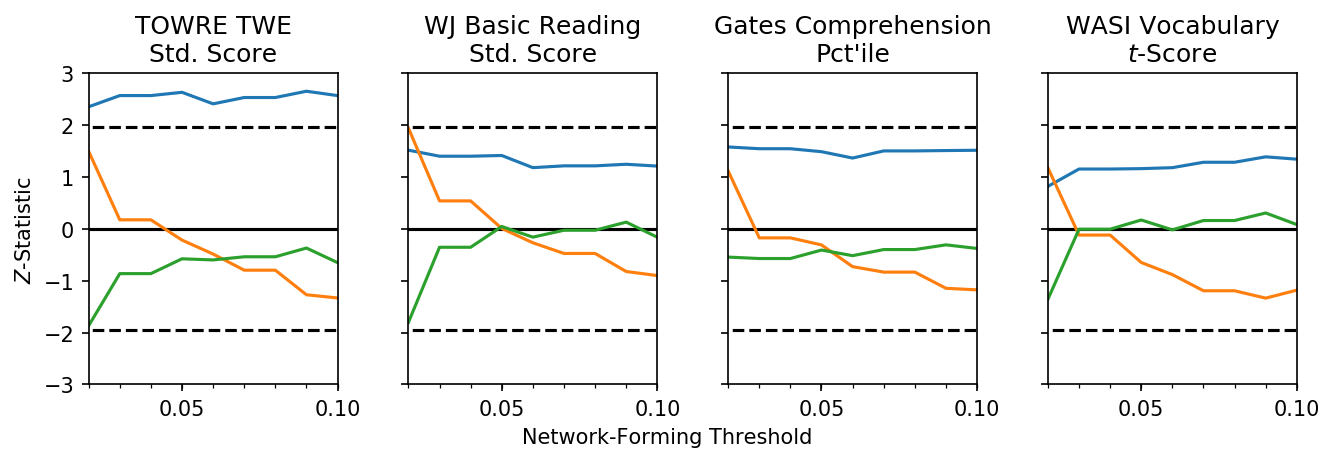
\includegraphics[width=5.5in]{ch2-global-glm-covariates-thresholds}
    \caption[Modularity metrics at rest are the best predictors of cognitive skills.] {Global modularity was the most stable and predictive network measure for predicting language-related skills, although it only reached significance thresholds for the TOWRE.}
    \label{fig:ch2-global-glm-covariates-thresh}
\end{figure}

Finally, we investigated the correlation between each individual RSN's modularity contribution and TOWRE scores (Fig. \ref{fig:ch2-rsn-node-modularity-corr}). Overall, no RSN reached the strength of correlation of the global modularity measure (i.e., $r = 0.378$). The default mode RSN had the highest correlation with the TOWRE ($r_{DMN} = 0.350$), with the memory retrieval ($r_{MEM} = 0.303$) and attention ($r_{DAN} = 0.236$, $r_{VAN} = 0.248$) RSNs ranking next. Interestingly, the relationship was inverted in the auditory and cingulo-opercular RSNs: lower modularity was associated with better reading skill ($r = -0.178$).

\begin{figure}[t]
    \centering
    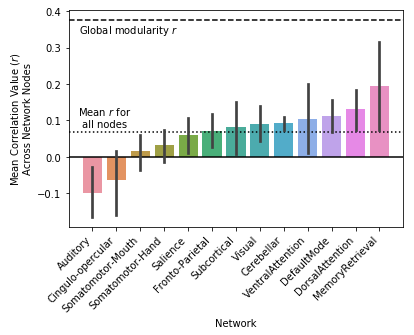
\includegraphics[height=3in]{ch2-rsn-node-modularity-corr}
    \caption[Modularity relationship with TOWRE varies by RSN.] {Modularity relationship with TOWRE varies by RSN. Although no individual RSN matched the strength of correlation of the global modularity measure, the default mode and memory retrieval RSNs had significant positive correlations with the TOWRE. The auditory and cingulo-opercular RSNs, on the other hand, had significant negative correlations.}
    \label{fig:ch2-rsn-node-modularity-corr}
\end{figure}

\section{Discussion}

% Review of findings
Our aim for Study 1 was to establish whether network measures of resting-state fMRI data were related to reading skill. We established a series of methods and measures for summarizing the global and RSN-level network architecture, and showed that of all metrics, modularity was most robustly able to index reading skill in our sample. We also explored how variations of this measure among RSNs is associated with individual differences in reading ability. This demonstrated that modularity within the default mode network is most similar to the modularity of the whole brain, and it also revealed significant negative correlations between the modularity of the auditory and cingulo-opercular networks and reading skill.

% Significance of graph theory descriptions
One advantage to our approach is that we used an \textit{a priori} defined set of nodes and network parcellation \citep{Power2013}. We then employed standard measures that are sensitive to RSN properties: modularity, participation coefficient and path length. Although adjusting the network-forming threshold had a sizable impact on the values yielded for each metric, the relative contributions of each RSN to each metric were fairly stable. That is, there was a global and not local trend in the effect of thresholds, with a few exceptions for very small RSNs (for example, the memory retrieval network). Modularity, in particular, was relatively stable across thresholds, as indicated by its consistent relationship to cognitive metrics (Fig. \ref{fig:ch2-global-glm-covariates-thresh}).

% Significance of global findings
Modularity was the most effective measure for predicting individual differences, especially in reading but more broadly in verbal skill. Modularity is a measure of network segregation: the more different each RSN behaves during rest, the higher the modularity will be. One possible explanation is that modularity is an essential component to the entire network organization, whereas participation coefficient and path length are more regionally variable throughout the network \citep{Bullmore2012}. Furthermore, this finding is consistent with previous literature showing that anti-correlations between the default mode network and the fronto-parietal network index cognitive skills \citep{Anticevic2012}. 

% Significance of RSN findings
The regional variability in correlation strength was also notable. We were surprised to find an anti-correlation between modularity in the auditory and cingulo-opercular networks and reading skill, given the global trend of positive correlations. (The bootstrapped distribution yielded a range of correlation values spanning approximately $r = 0.0$ to $r = 0.4$. See Fig \ref{fig:ch2-rsn-node-modularity-corr}.) The localization of these differences onto the auditory network support a hypothesis that, in better readers, auditory networks are more integrated with other networks, such as visual networks. Although the modularity measure cannot support this directly, follow-up studies investigating task differences may be able to do. On the other end, we found that the default mode network was most highly correlated with reading and most closely approximated the global correlation. The DMN supports a wide range of cognitive processes important for comprehension, including theory of mind, narrative processing, and autobiographical recall \citep{Buckner2008, AbdulSabur2014}, and its cohesiveness during resting-state has been used to investigate other disorders \citep{Uddin2008}. 

% Significance of modularity
Modularity in biological systems is an important feature from an evolutionary standpoint. It increases adaptability and robustness and thus increases the system's evolvability \citep{Sporns2016}. Although no consensus interpretation exists, one could speculate that increased modularity indexes segregation of functions. This interpretation stems from a wide range of studies showing opposing activation in externally directed cognitive tasks for the fronto-parietal and default RSNs, during which functions of the two networks ought to be segregated to prevent interference \citep{Reineberg2018}. That is, an increase in modularity indicates that each RSN is more capable of functioning independently, without the participation of external regions. Future studies will have to investigate this directly.

% Limitations of the present approach
While this study is one of the first to examine the relationship between reading skills and intrinsic network architecture, there are a few limitations. One limitation is the extent of inference we can make about specific behavioral skills. We used a composite measure of reading that accounts for phonological decoding and sight-word reading skill, but reading skill relies on a number of other processes (e.g. semantic processing). Due to shared variance between these measures -- and even domain-general ones -- it is difficult to pinpoint which cognitive process is most closely associated with modularity. However, the finding that modularity was more closely associated with Sight Word Efficiency (which requires no decoding) than Phonemic Decoding Efficiency provides some evidence that modularity is related to speed of transfer of information between different systems, rather than environmental tuning. Another limitation is that, because we examined these relationships in relatively mature readers, it is possible that other relationships might be observed in developing readers. Such processes explain less and less variance in reading skill as texts become more difficult and reading starts to reach mature levels \citep{Cutting2006a}. 

% Conclusions
Overall, the current results demonstrate that modularity is an important indicator of successful reading skill, and there appear to be regional variations which influence it. Future work will need to examine not just the internal connectivity, but the relationships between these networks during reading and at rest. The default mode network, for example, is typically anti-correlated with ``task-positive'' networks such as the fronto-parietal network. A high degree of anti-correlation has been reported to be important for performance on a variety of cognitive processes \citep{Fox2005, Keller2015}, but recent work suggests that high modularity and connectivity of the default mode during higher-level cognition is fundamental to processes relying on self-referential and memory retrieval processes, such as those found in language \citep{Vatansever2015}. How this modular architecture changes during the reading process is an important question that we will tackle in the following chapter. 
